\PassOptionsToPackage{unicode=true}{hyperref} % options for packages loaded elsewhere
\PassOptionsToPackage{hyphens}{url}
%
\documentclass[12pt,]{article}
\usepackage{lmodern}
\usepackage{amssymb,amsmath}
\usepackage{ifxetex,ifluatex}
\usepackage{fixltx2e} % provides \textsubscript
\ifnum 0\ifxetex 1\fi\ifluatex 1\fi=0 % if pdftex
  \usepackage[T1]{fontenc}
  \usepackage[utf8]{inputenc}
  \usepackage{textcomp} % provides euro and other symbols
\else % if luatex or xelatex
  \usepackage{unicode-math}
  \defaultfontfeatures{Ligatures=TeX,Scale=MatchLowercase}
\fi
% use upquote if available, for straight quotes in verbatim environments
\IfFileExists{upquote.sty}{\usepackage{upquote}}{}
% use microtype if available
\IfFileExists{microtype.sty}{%
\usepackage[]{microtype}
\UseMicrotypeSet[protrusion]{basicmath} % disable protrusion for tt fonts
}{}
\IfFileExists{parskip.sty}{%
\usepackage{parskip}
}{% else
\setlength{\parindent}{0pt}
\setlength{\parskip}{6pt plus 2pt minus 1pt}
}
\usepackage{hyperref}
\hypersetup{
            pdfborder={0 0 0},
            breaklinks=true}
\urlstyle{same}  % don't use monospace font for urls
\usepackage[margin=1in]{geometry}
\usepackage{longtable,booktabs}
% Fix footnotes in tables (requires footnote package)
\IfFileExists{footnote.sty}{\usepackage{footnote}\makesavenoteenv{longtable}}{}
\usepackage{graphicx,grffile}
\makeatletter
\def\maxwidth{\ifdim\Gin@nat@width>\linewidth\linewidth\else\Gin@nat@width\fi}
\def\maxheight{\ifdim\Gin@nat@height>\textheight\textheight\else\Gin@nat@height\fi}
\makeatother
% Scale images if necessary, so that they will not overflow the page
% margins by default, and it is still possible to overwrite the defaults
% using explicit options in \includegraphics[width, height, ...]{}
\setkeys{Gin}{width=\maxwidth,height=\maxheight,keepaspectratio}
\setlength{\emergencystretch}{3em}  % prevent overfull lines
\providecommand{\tightlist}{%
  \setlength{\itemsep}{0pt}\setlength{\parskip}{0pt}}
\setcounter{secnumdepth}{5}
% Redefines (sub)paragraphs to behave more like sections
\ifx\paragraph\undefined\else
\let\oldparagraph\paragraph
\renewcommand{\paragraph}[1]{\oldparagraph{#1}\mbox{}}
\fi
\ifx\subparagraph\undefined\else
\let\oldsubparagraph\subparagraph
\renewcommand{\subparagraph}[1]{\oldsubparagraph{#1}\mbox{}}
\fi

% set default figure placement to htbp
\makeatletter
\def\fps@figure{htbp}
\makeatother

\usepackage{booktabs}
\usepackage{longtable}
\usepackage{array}
\usepackage{multirow}
\usepackage{wrapfig}
\usepackage{float}
\usepackage{colortbl}
\usepackage{pdflscape}
\usepackage{tabu}
\usepackage{threeparttable}
\usepackage{threeparttablex}
\usepackage[normalem]{ulem}
\usepackage{makecell}
\definecolor{Blue}{rgb}{0.01,0.28,1.0}
\definecolor{Maroon}{rgb}{0.5,0.0,0.0}
\definecolor{darkgreen}{RGB}{0,150,0}
\hypersetup{colorlinks=true, citecolor=Blue, urlcolor=Maroon}
\renewcommand{\thetable}{S\arabic{table}} 
\renewcommand{\thefigure}{S\arabic{figure}}
\usepackage[]{natbib}
\bibliographystyle{bib/jae.bst}

\author{}
\date{\vspace{-2.5em}}

\begin{document}

\renewcommand{\bibsection}{}  %% No section name for bibliography

\begin{center}
  \Large{\textbf{SUPPLEMENTARY MATERIALS}}
\end{center}

\vspace{1cm}

\begin{center}
  \LARGE{Spatial forecasting of tropical moist forest cover change in the 21$^{\text{st}}$ century}
\end{center}

\vspace{1cm}

\begin{center}
  \large{
  Ghislain VIEILLEDENT$^{[1, 2, 3, 4, \star]}$ \hspace{0.5cm} Christelle VANCUTSEM$^{[1]}$\\
  \vspace{0.5cm}
  and \hspace{0.5cm} Frédéric ACHARD$^{[1]}$
  }
\end{center}

\vspace{1cm}

{\small
  \begin{flushleft}  
    $[1]$ \textbf{European Commission}, JRC, Bio-economy Unit, I-21027 Ispra (VA), ITALY\\
    $[2]$ \textbf{CIRAD}, UPR Forêts et Sociétés, F-34398 Montpellier, FRANCE\\
    $[3]$ \textbf{CIRAD}, UMR AMAP, F-34398 Montpellier, FRANCE\\
    $[4]$ AMAP, \textbf{Univ Montpellier}, CIRAD, CNRS, INRAE, IRD, Montpellier, FRANCE\\
    ~\\
    $[\star]$ \textbf{Corresponding author:}
    \textbackslash{E-mail}:~ghislain.vieilledent@cirad.fr
    \textbackslash{Phone}:~+33 4 67 61 49 09\\
  \end{flushleft}}

\newpage

\newpage

\hypertarget{materials-and-methods}{%
\section{Materials and Methods}\label{materials-and-methods}}

\hypertarget{study-areas}{%
\subsection{Study areas}\label{study-areas}}

We defined 119 study areas representing 92 countries (Table~\ref{tab:samp-size}) and covering the integrality of the moist tropical forest in the world, at the exception of some islands (eg. Sao Tome and Principe or Wallis-and-Futuna). Each country was identified by one unique three-letter code following the ISO 3166-1 standard (eg. MDG for Madagascar or GUF for French Guyana). Most of the countries corresponded to one unique study area, with three exceptions: Brazil, India, and Australia. Brazil, because of its large size, was divided into 26 study areas corresponding to the 26 administrative states (the state of Goias including the Federal District). For India, which is also a large country, the tropical moist forest is located in three distinct regions far from each other. We thus considered three independent study areas for India: the Western Ghats, North-East India (including the West Bengale), and the union territory of the Andaman and Nicobar Islands. For Australia, we only considered the Queensland state as a study area. Data sampling and spatial deforestation modelling were performed independently for each study area. Study area borders were obtained from version 3.6 of the Global Administrative Areas database (\url{https://gadm.org}). We used level-0 data for study areas corresponding to countries and level-1 data for study areas corresponding to states or regions. We grouped the study areas in three continents (Fig.~\ref{fig:study-areas}): America (64 study areas for 39 countries), Africa (32 study areas for 32 countries), and Asia (23 study areas for 21 countries).

\hypertarget{historical-forest-cover-change-maps}{%
\subsection{Historical forest cover change maps}\label{historical-forest-cover-change-maps}}

For each study area, we derived historical forest cover change maps on two periods of time: 1\(^{\text{st}}\) January 2000 -- 1\(^{\text{st}}\) January 2010, and 1\(^{\text{st}}\) January 2010 -- 1\(^{\text{st}}\) January 2020 from the forest cover change annual product by \citet{Vancutsem2020}. The annual product by \citet{Vancutsem2020} classifies Landsat image pixels at 30~m resolution in 16 categories for each year (on the 31\(^{\text{st}}\) of December) between 1982 and 2019 and allows identifying moist tropical forest pixels at each date (Table~\ref{tab:cat-annual-product}). This classification is based on an expert model analyzing time-series data at the pixel level extracted from the full Landsat satellite image archive on the period 1982--2019. The expert model has been built on Google Earth Engine \citep{Gorelick2017}. For our forest definition, we only considered natural old-growth moist tropical forest, disregarding plantations and regrowths. We included degraded forests (not yet deforested) in our forest definition. As a consequence, we considered pixels in the following categories: 1, 2, 3, 4, 5, 13, or 14 in the annual product, to be natural old-growth moist tropical forest pixels (simply abbreviated ``forest'' in this manuscript). Because several decades are usually necessary to reach the state of old-growth forest, we assumed every pixels classified as ``forest'' at a given date between 1999 and 2019 to be also classified as ``forest'' in the previous years of that period of time. We thus obtained three forest cover maps for the dates 1\(^{\text{st}}\) January 2000, 1\(^{\text{st}}\) January 2010, and 1st January 2020. We combined these three maps to obtained high-resolution moist tropical forest cover change maps on the periods 2000--2010--2020 at 30~m resolution at the global scale.

We did not consider potential forest regrowth in our forest definition for three main reasons. First, throughout the humid tropics, forest regeneration involves much smaller areas than deforestation \citep[see also 2000-2012 tree cover gain in \citet{Hansen2013}]{Vancutsem2020}. Second, there is little evidence of natural forest regeneration in the long term in the tropics \citep{Grouzis2001}. This can be explained by several ecological processes following deforestation such as soil erosion \citep{Grinand2017} and reduced seed bank due to fire-induced deforestation and soil loss \citep{Grouzis2001}. Moreover, in areas where forest regeneration is ecologically possible, young forest regrowth are more easily re-burnt for agriculture and pasture \citep{Vieilledent2020}. Third, young secondary forests generally provide more limited ecosystem services compared to old-growth natural forests in terms of biodiversity \citep{Gibson2011} and carbon storage \citep{Blanc2009}.

\textbf{Add a figure for forest cover and indicate web-site with interactive map.}

\hypertarget{spatial-explanatory-variables}{%
\subsection{Spatial explanatory variables}\label{spatial-explanatory-variables}}

To explain the observed deforestation on the period 2010--2020, we considered a set of spatial explanatory variables describing: topography (altitude and slope), accessibility (distances to nearest road, town, and river), forest landscape (distance to forest edge), deforestation history (distance to past deforestation), and land conservation status (presence of a protected area). This set of variables were selected on an \emph{a priori} knowledge of the deforestation process \citep{Gorenflo2011, Vieilledent2013, Geist2001}. For example, the risk of deforestation is supposed to decrease with the distance to road and forest edge (lower accessibility), to increase at lower elevation and slope (higher probability to find arable lands), and to decrease in protected areas (higher level of protection). Characteristics of each explanatory variable are summarized in Table~\ref{tab:variables}.

Elevation (in m) and slope (in degree) at 90~m resolution were obtained from the SRTM Digital Elevation Database v4.1 (\url{http://srtm.csi.cgiar.org/}). Distances (in m) to nearest road, town and river at 150~m resolution were obtained from the OpenStreetMap (OSM) project (\url{https://www.openstreetmap.org/}). OSM country data were downloaded from two web-sites: Geofabric (\url{http://download.geofabrik.de/}) and OpenStreetMap.fr (\url{https://download.openstreetmap.fr/extracts/}) depending on the availability of the data for each country. To obtain the road network in each country, we considered the ``motorway'', ``trunk'', ``primary'', ``secondary'' and ``tertiary'' categories for the ``highway'' key in OSM. To obtain the network of populated places in each country (that we simply call ``towns'' in the present study), we considered the ``city'', ``town'' and ``village'' categories for the ``place'' key in OSM. To obtain the river network in Madagascar, we considered the ``river'' and ``canal'' categories for the ``waterway'' key in OSM. For a more detailed description of each category, see the OSM wiki page (\url{https://wiki.openstreetmap.org/wiki/Tags}). OSM data have been downloaded during the period January--March 2020 for all countries. Distance to forest edge was computed at 30~m resolution from the forest cover map in 2010. Distance to past deforestation in 2010 was computed at 30~m resolution from the 2000--2010 forest cover change map. To minimize border effect for the computation of distance to forest edge and distance to past deforestation, a buffer of 10~km around each study area extent was considered. Data on protected areas were obtained from the World Database on Protected Areas (\url{https://www.protectedplanet.net}, \citet{WDPA2020}) using the \texttt{pywdpa} Python package (\url{https://pypi.org/project/pywdpa/}). WDPA data have been downloaded during the period January--March 2020 for all countries. All protected areas defined by at least one polygon were considered in the analysis, but protected areas defined by a point were not taken into account. Data included protected areas of all IUCN~categories (from Ia to VI) and of all types defined at the national level (e.g.~National Parks, Reserves), even if the type and IUCN category were not reported. Polygons representing protected areas were rasterized at 30~m resolution.

In total, we obtained 8 spatial explanatory variables to model the spatial probability of deforestation Table~\ref{tab:variables}.

\textbf{Add figures for explanatory variables: global road network, global protected areas.}

\hypertarget{data-sampling-for-spatial-modelling-of-the-deforestation}{%
\subsection{Data sampling for spatial modelling of the deforestation}\label{data-sampling-for-spatial-modelling-of-the-deforestation}}

Through the spatial modelling of the deforestation, our aim was not to estimate the intensity of the deforestation (or ``quantity'' census \citet{Pontius2011}), that could be expressed in \%/year or in ha/year for example. With our spatial model, our aim was to estimate the effects of a set of variables in determining the location of the deforestation (or ``allocation'' census \citet{Pontius2011}) and compute the relative probability of deforestation for each forest pixels. A balanced sampling between deforested and non-deforested pixels is preferable in this case \citep{Dezecache2017, Vieilledent2013}. Because deforestation events are rare (\(\approx\) 1~\%/yr), a non-stratified random sampling would lead to very few observations of deforestation events, rendering difficult a good estimation of the effects of the explanatory variables. Stratified balanced sampling provided non-biased estimates of the model's parameters, except for the model's intercept (estimated average deforestation). Having a biased model intercept (which has the same value for all forest pixels) is not a problem as we are interested in estimating a \emph{relative} probability of deforestation for all forest pixels.

As a consequence, we performed a stratified balanced sampling between (i) forest pixels in 2010 which have been deforested on the period 2010--2020 (``deforested'' pixels), and (ii) forest pixels in 2010 which have not been deforested on that period of time and which represent the remaining forest in 2020 (``non-deforested'' pixels). Forest pixels in each category were sampled randomly. To maximize the representativity of the data, the total number of forest pixels sampled in each study area for the year 2010 was chosen proportional to the area of forest in 2010 in that study area (2000 points for 1~Mha of forest), with the condition that this number had to be between 20,000 (to be representative of the deforestation process) and 100,000 (to limit computation time). When, for a specific study area, the total number of pixels in one of the two categories (deforested vs.~non-deforested pixels) was \(\leq\) 10,000, all the pixels of that category were included in the sample. This could happen for study areas with low moist forest cover such as small islands (eg. Antigua and Barbuda). For each sampled pixel, we retrieved information regarding the 8 computed explanatory variables at their original spatial resolution. When the information was not complete for a given pixel (eg. elevation and slope data missing for a forest pixel located close to the sea border), the observation was removed from the data-set. Missing information affected a minority of pixels. The global data-set included a total of 3,186,698 observations (1,601,810 of non-deforested pixels and 1,584,888 of deforested pixels, corresponding to an area of 144,163~ha and 142,647~ha, respectively).

\textbf{Add figure for data sampling (red and green points).}

\hypertarget{spatial-deforestation-model}{%
\subsection{Spatial deforestation model}\label{spatial-deforestation-model}}

Using observations of the deforestation on the period 2010--2020, we modelled the spatial probability of deforestation as a function of the 8 explanatory variables using a logistic regression. We considered the random variable \(y_i\) which takes value 1 if the forest pixel \(i\) was deforested on the period 2010--2020 and 0 if it was not. We assumed that \(y_i\) follows a Bernoulli distribution of parameter \(\theta_i\). In our model, \(\theta_i\) represents the spatial probability of deforestation for pixel \(i\). We assumed that \(\theta_i\) is linked, through a logit function, to a linear combination of the explanatory variables \(X_i \beta\), where \(X_i\) is the vector of explanatory variables for pixel \(i\), and \(\beta\) is the vector of effects \([\beta_1, \ldots, \beta_8]\) of each variable to be estimated. All the continuous explanatory variables were normalized before fitting the model. The model includes an intercept \(\alpha\). To account for the residual spatial variation in the deforestation process, we included an additional random effect \(\rho_{j(i)}\) for each spatial cell \(j\) of a 10 \(\times\) 10~km grid covering each study area. This grid resolution was choosen in order to have a reasonable balance between a good representation of the spatial variability of the deforestation process and the number of parameters. A forest pixel \(i\) was associated to one cell \(j\) and one random effect \(\rho_{j(i)}\). We assumed that random effects were spatially autocorrelated through an intrinsic conditional autoregressive (iCAR) model \citep{Besag1991, Banerjee2014}. This model is denoted ``icar'' in subsequent sections and results. In an iCAR model, the random effect \(\rho_j\) associated to cell \(j\) depends on the values of the random effects \(\rho_{j^{\prime}}\) associated to neighbouring cells \(j^{\prime}\). In our case, the neighbouring cells are connected to the target cell \(j\) through a common border or corner (cells defined by the ``king move'' in chess, See Fig. X). The variance of the spatial random effects \(\rho_j\) was denoted \(V_{\rho}\). The number of neighbouring cells for cell \(j\), which might vary, was denoted \(n_j\). Additional spatial random effects \(\rho_j\) account for unmeasured or unmeasurable variables \citep{Clark2005} that explain a part of the residual spatial variation in the deforestation process that is not explained by the fixed spatial explanatory variables (\(X_i\)).

\begin{equation}
\begin{split}
  y_i \sim \mathcal{B}ernoulli(\theta_i)\\
  \text{logit}(\theta_i) = \alpha + X_i \beta + \rho_{j(i)}\\
  \rho_{j(i)} \sim \mathcal{N}ormal(\sum_{j^{\prime}} \rho_{j^{\prime}} / n_j,V_{\rho} / n_j)
\end{split}
\label{eq:icar}
\end{equation}

\textbf{Add figure for CAR model (damier).}

\textbf{Add figure for the grid over a country, e.g.~DRC.}

\hypertarget{variable-selection}{%
\subsection{Variable selection}\label{variable-selection}}

Variable selection was performed using a backward elimination procedure. All the spatial explanatory variables in our data-set should decrease the deforestation risk (having a negative effect on the probability of deforestation). For example, the probability of deforestation should decrease with the distance to forest edge and should also decrease inside a protected area. Our variable selection procedure was thus not based on statistical significance but on background knowledge regarding the deforestation process and on the interpretabiliy of the variable effects \citep{Heinze2018}. For each study area, we started to fit a model with the full set of explanatory variables (8 variables). At each step of the procedure, we removed the variables having a positive effect on the probability of deforestation. This was done in order to avoid unrealistic predictions of the spatial probability of deforestation at the study area scale. For example, it is not realistic to observe, at a country scale, a decrease of the deforestation with the distance to forest edge (higher deforestation risk in the core of the forest compared with forest edge). This might happen in a particular context for a very specific region but is very unlikely at a country scale. In most of the case, when we found a positive effect for a given explanatory variable, it was non-significant (95\% credible inteval including zero). On the contrary, when whe found a negative but non-significant effect for a given explanatory variable, we kept this variable in the model. This effect, albeit non-significant, was interpretable given our background knowledge of the deforestation process and was relatively lower than the effect of the other variables.

\hypertarget{parameter-inference}{%
\subsection{Parameter inference}\label{parameter-inference}}

Parameter inference was done in a hierarchical Bayesian framework. Non-informative priors were used for all parameters: \(\alpha \sim \mathcal{N}ormal(\text{mean}=0,\text{var}=10^6)\), \(\beta \sim \mathcal{N}ormal(\text{mean}=0,\text{var}=10^6)\), and \(V_{\rho} \sim 1/\mathcal{G}amma(\text{shape}=0.05,\text{rate}=0.0005)\). During the variable selection procedure, we run a Markov Chain Monte Carlo (MCMC) of 2000 iterations, discarding the first 1000 iterations (burn-in phase). For the final model, we repeated the parameter inference using a longer MCMC of 10,000 iterations. We discarded the first 5000 iterations (burn-in phase), and we thinned the chain each 5 iterations (to reduce autocorrelation between samples). We obtained 1000 estimates for each parameter. MCMC convergence was visually checked looking at MCMC traces and parameter posterior distributions. Function \texttt{model\_binomial\_iCAR()} from the \texttt{forestatrisk} Python package was used for parameter inference. This function calls an adaptive Metropolis-within-Gibbs algorithm \citep{Rosenthal2011} written in C for maximum computation speed.

\textbf{Add figure for MCMC traces (see bayesplot).}

\hypertarget{model-comparison}{%
\subsection{Model comparison}\label{model-comparison}}

We computed the deviance \(\mathcal{D}\) of the two models with the formula \(\mathcal{D}=-2 \log \mathcal{L}\), \(\mathcal{L}\) being the likelihood of the model, i.e.~the probability of observing the data given the model and estimated parameters. We compared the deviance of the two models with the deviances of both the ``null'' model and the ``full'' model. The ``null'' model assumes a constant probability of deforestation for all theobservations and has only one parameter, the intercept of the linear relationship. At the other extreme, the ``full'' model has as many parameters as there are observations. We then computed the percentage of deviance explained by each model, considering that the ``null'' model explains 0\% of the deviance and the ``full'' model explains 100\% of the deviance.

We also performed a cross-validation to compare models using an independent validation data-set of 20,000 forest pixels in 2000. Again, the sample was stratified between 10,000 deforested pixels in 2000--2010 and 10,000 non-deforested pixels. We used the fitted models to predict the deforestation probability of all the pixels of the validation data-set. To transform the deforestation probabilities into binary values, we identified the probability threshold respecting the percentage of deforested pixels (eg. the mode of the probabilities for a deforestation rate of 50\%). Using model predictions and observations, we computed several accuracy indices: the Area Under the ROC Curve (AUC), the Figure of Merit (FOM), the Overall Accuracy (OA), the Expected Accuracy (EA), the Kappa of Cohen (K), the Specificity (Spe), the Sensitivity(Sen), and the True Skill Statistics (TSS). A detailed description of these indices can be found in \citet{Pontius2008} (for the FOM) and \citet{Liu2011} (for all the other indices). Formulas used to compute these indices are presented in Appendix~1.

Because the value of these indices depends on the deforestation rate \citep{Pontius2008}, we computed the accuracy indices for various percentage of deforested pixels: 1, 5, 10, 25 and 50\%. To do so, we selected subsamples of the deforested pixels in our validation data-set at random.

\hypertarget{computing-the-spatial-probability-of-deforestation-in-2010}{%
\subsection{Computing the spatial probability of deforestation in 2010}\label{computing-the-spatial-probability-of-deforestation-in-2010}}

For the ``icar'' model, before computing the predictions of the deforestation probability, the spatial random effects at 10~km were interpolated at 1~km using a bicubic interpolation method. This was done in order to obtain spatial random effects at a resolution closer to the original forest raster resolution of 30~m, and to smooth the deforestation probability spatially.

Deforestation probabilities (float values in the interval \([0, 1]\)) were transformed as integer values on the interval \([\![1, 65535]\!]\). This allowed us to record the large raster of probabilities as UInt16 type and save space on disk. We then obtained a map of the relative probability of deforestation for the year 2010 at 30~m resolution.

In 2010, Madagascar was covered by 9.3~Mha of natural forest corresponding to more than 104~M pixels at 30~m resolution. Predictions were computed using functions \texttt{predict\_raster*()} from the \texttt{forestatrisk} Python package which make computation fast and efficient (with low memory usage) by treating raster data by blocks.

\hypertarget{forecasting-forest-cover-change-on-the-period-20102017}{%
\subsection{Forecasting forest cover change on the period 2010--2017}\label{forecasting-forest-cover-change-on-the-period-20102017}}

We computed the observed deforestation \(D\) (in ha) on the period 2010--2017 from the forest cover maps at these two dates. To forecast the forest cover change in 2010--2017 with our models, we used the previously derived maps of relative probability of deforestation in 2010. The resolution of these maps is \(r=30\)~m, equivalent to \(r_{\text{ha}}=0.09\)~ha. We computed a probability threshold \(\theta_T\) in the interval \([\![1, 65535]\!]\) identifying the \(n\) forest pixels in 2010 with the highest probability of deforestation so that \(n r_{\text{ha}} = D + \epsilon\). Because deforestation probabilities have finite values in \([\![1, 65535]\!]\), some forest pixels might have the same deforestation probability and it might not be possible to identify \(\theta_T\) such that \(\epsilon=0\). We thus selected the threshold \(\theta_T\) minimizing \(\epsilon\). We obtained negligible \(\epsilon\) (\(<\) 32,000~ha) compared to \(D\) (874,211~ha) for both models. We considered those \(n\) forest pixels in 2010 as deforested on the period 2010--2017 and derived the forest cover change map on that period.

\hypertarget{softwares}{%
\subsection{Softwares}\label{softwares}}

\newpage

\hypertarget{tables}{%
\section{Tables}\label{tables}}

\hypertarget{categories-of-the-forest-cover-annual-product}{%
\subsection{Categories of the forest cover annual product}\label{categories-of-the-forest-cover-annual-product}}



\begin{table}[H]

\caption{\label{tab:cat-annual-product}\textbf{Categories of the forest cover annual product by \citet{Vancutsem2020}}. The forest cover annual product classifies Landsat image pixels in 16 categories for each year (on the 31\(^{\text{st}}\) of December) between 1982 and 2019 and allows identifying moist tropical forest pixels at each date. Water data comes from \citet{Pekel2016}.\vspace{0.5cm}~}
\centering
\begin{tabular}[t]{>{\raggedright\arraybackslash}p{2cm}>{\raggedleft\arraybackslash}p{10cm}}
\toprule
Class & Definition\\
\midrule
\rowcolor{gray!6}  1 & Tropical moist forest (TMF including bamboo-dominated forest and mangroves)\\
2 & TMF converted later in a tree plantation\\
\rowcolor{gray!6}  3 & NEW degradation\\
4 & Ongoing degradation (disturbances still detected)\\
\rowcolor{gray!6}  5 & Degraded forest (former degradation, no disturbances detected anymore)\\
6 & NEW deforestation (may follow degradation)\\
\rowcolor{gray!6}  7 & Ongoing deforestation (disturbances still detected)\\
8 & NEW Regrowth\\
\rowcolor{gray!6}  9 & Regrowthing\\
10 & Other land cover (not water)\\
\rowcolor{gray!6}  11 & Permanent Water (Pekel et al. 2016)\\
12 & Seasonal Water (Pekel et al. 2016)\\
\rowcolor{gray!6}  13 & Init period without valid data - Init class = TMF\\
14 & Init period with min 1 valid obs - Init class = TMF\\
\rowcolor{gray!6}  15 & Nodata - Init class = other LC\\
16 & Init period without valid data - Init class = Plantation\\
\bottomrule
\end{tabular}
\end{table}

\hypertarget{variables}{%
\subsection{Variables}\label{variables}}



\begin{table}[H]

\caption{\label{tab:variables}\textbf{Set of explicative variables used to model the spatial probability of deforestation}. A total of height variables were tested. They indicate topography, forest accessibility, forest landscape, deforestation history, and conservation status.\vspace{0.5cm}~}
\centering
\begin{tabular}[t]{>{\raggedright\arraybackslash}p{3cm}>{\raggedright\arraybackslash}p{3cm}>{\raggedright\arraybackslash}p{3cm}>{\raggedleft\arraybackslash}p{2cm}>{\raggedleft\arraybackslash}p{2cm}r}
\toprule
Product & Source & Variable derived & Unit & Resolution (m) & Date\\
\midrule
\rowcolor{gray!6}  Forest maps (2000-2010-2020) & Vancutsem et al. 2020 & distance to forest edge & m & 30 & --\\
 &  & distance to past deforestation & m & 30 & --\\
\rowcolor{gray!6}  Digital Elevation Model & SRTM v4.1 CSI-CGIAR & altitude & m & 90 & --\\
 &  & slope & degree & 90 & --\\
\rowcolor{gray!6}  Highways & OSM-Geofabrik & distance to roads & m & 150 & Jan-Mar 2020\\
Places &  & distance to towns & m & 150 & Jan-Mar 2020\\
\rowcolor{gray!6}  Waterways &  & distance to river & m & 150 & Jan-Mar 2020\\
Protected areas & WDPA & presence of protected area & -- & 30 & Jan-Mar 2020\\
\bottomrule
\end{tabular}
\end{table}

\hypertarget{sample-size}{%
\subsection{Sample size}\label{sample-size}}



\begingroup\fontsize{10}{12}\selectfont

\begin{longtable}[t]{llrrrr}
\caption{\label{tab:samp-size}\textbf{Number of observations used for the spatial model of deforestation for each study area}. The table includes the number of non-deforested (nfor) and deforested (ndef) pixels per study area. These numbers include the forest pixels with full information regarding the explanatory variables. The corresponding number of hectares is also provided (nfHa and ndHa, respectively).\vspace{0.5cm}~}\\
\toprule
Continent & iso3 & nfor & ndef & nfHa & ndHa\\
\midrule
\rowcolor{gray!6}  Africa & AGO & 10,000 & 10,000 & 900 & 900\\
Africa & BDI & 10,000 & 9,999 & 900 & 900\\
\rowcolor{gray!6}  Africa & BEN & 9,981 & 9,995 & 898 & 900\\
Africa & CAF & 10,000 & 10,000 & 900 & 900\\
\rowcolor{gray!6}  Africa & CIV & 10,000 & 10,000 & 900 & 900\\
Africa & CMR & 22,983 & 22,987 & 2,068 & 2,069\\
\rowcolor{gray!6}  Africa & COD & 50,000 & 50,000 & 4,500 & 4,500\\
Africa & COG & 23,412 & 23,411 & 2,107 & 2,107\\
\rowcolor{gray!6}  Africa & COM & 9,990 & 9,984 & 899 & 899\\
Africa & ETH & 10,000 & 10,000 & 900 & 900\\
\rowcolor{gray!6}  Africa & GAB & 23,986 & 23,966 & 2,159 & 2,157\\
Africa & GHA & 9,999 & 10,000 & 900 & 900\\
\rowcolor{gray!6}  Africa & GIN & 9,978 & 9,998 & 898 & 900\\
Africa & GMB & 9,988 & 9,999 & 899 & 900\\
\rowcolor{gray!6}  Africa & GNB & 9,882 & 9,977 & 889 & 898\\
Africa & GNQ & 9,997 & 9,988 & 900 & 899\\
\rowcolor{gray!6}  Africa & KEN & 9,986 & 9,998 & 899 & 900\\
Africa & LBR & 9,999 & 9,997 & 900 & 900\\
\rowcolor{gray!6}  Africa & MDG & 9,994 & 9,998 & 899 & 900\\
Africa & MUS & 9,968 & 9,969 & 897 & 897\\
\rowcolor{gray!6}  Africa & MWI & 10,000 & 10,000 & 900 & 900\\
Africa & MYT & 9,963 & 9,983 & 897 & 898\\
\rowcolor{gray!6}  Africa & NGA & 9,984 & 9,995 & 899 & 900\\
Africa & REU & 9,996 & 9,995 & 900 & 900\\
\rowcolor{gray!6}  Africa & RWA & 10,000 & 10,000 & 900 & 900\\
Africa & SEN & 9,892 & 9,976 & 890 & 898\\
\rowcolor{gray!6}  Africa & SLE & 9,997 & 9,999 & 900 & 900\\
Africa & SSD & 5,737 & 7,613 & 516 & 685\\
\rowcolor{gray!6}  Africa & TGO & 10,000 & 9,999 & 900 & 900\\
Africa & TZA & 9,983 & 9,970 & 898 & 897\\
\rowcolor{gray!6}  Africa & UGA & 10,000 & 10,000 & 900 & 900\\
Africa & ZMB & 10,000 & 10,000 & 900 & 900\\
\rowcolor{gray!6}  America & ATG & 9,840 & 6,336 & 886 & 570\\
America & BHS & 9,923 & 9,946 & 893 & 895\\
\rowcolor{gray!6}  America & BLZ & 9,995 & 9,999 & 900 & 900\\
America & BOL & 30,476 & 30,476 & 2,743 & 2,743\\
\rowcolor{gray!6}  America & BRB & 9,958 & 8,251 & 896 & 743\\
America & COL & 49,995 & 49,999 & 4,500 & 4,500\\
\rowcolor{gray!6}  America & CRI & 9,997 & 9,991 & 900 & 899\\
America & CUB & 9,955 & 9,958 & 896 & 896\\
\rowcolor{gray!6}  America & DMA & 9,991 & 9,878 & 899 & 889\\
America & DOM & 9,992 & 9,997 & 899 & 900\\
\rowcolor{gray!6}  America & ECU & 14,395 & 14,395 & 1,296 & 1,296\\
America & GLP & 9,979 & 9,923 & 898 & 893\\
\rowcolor{gray!6}  America & GRD & 9,974 & 9,928 & 898 & 894\\
America & GTM & 9,999 & 9,999 & 900 & 900\\
\rowcolor{gray!6}  America & GUF & 10,000 & 10,000 & 900 & 900\\
America & GUY & 18,511 & 18,511 & 1,666 & 1,666\\
\rowcolor{gray!6}  America & HND & 9,997 & 9,999 & 900 & 900\\
America & HTI & 9,952 & 9,970 & 896 & 897\\
\rowcolor{gray!6}  America & JAM & 9,988 & 9,996 & 899 & 900\\
America & KNA & 9,988 & 4,614 & 899 & 415\\
\rowcolor{gray!6}  America & LCA & 9,994 & 9,967 & 899 & 897\\
America & MAF & 3,156 & 3,808 & 284 & 343\\
\rowcolor{gray!6}  America & MEX & 9,994 & 9,997 & 899 & 900\\
America & MSR & 9,982 & 1,258 & 898 & 113\\
\rowcolor{gray!6}  America & MTQ & 9,972 & 9,973 & 897 & 898\\
America & NIC & 9,999 & 9,999 & 900 & 900\\
\rowcolor{gray!6}  America & PAN & 9,996 & 9,994 & 900 & 899\\
America & PER & 50,000 & 50,000 & 4,500 & 4,500\\
\rowcolor{gray!6}  America & PRI & 9,993 & 9,984 & 899 & 899\\
America & PRY & 10,000 & 10,000 & 900 & 900\\
\rowcolor{gray!6}  America & SLV & 9,965 & 9,982 & 897 & 898\\
America & SUR & 13,699 & 13,698 & 1,233 & 1,233\\
\rowcolor{gray!6}  America & SXM & 1,305 & 1,396 & 117 & 126\\
America & TTO & 9,993 & 9,984 & 899 & 899\\
\rowcolor{gray!6}  America & VCT & 9,981 & 9,792 & 898 & 881\\
America & VEN & 41,916 & 41,911 & 3,772 & 3,772\\
\rowcolor{gray!6}  America & VGB & 9,869 & 9,851 & 888 & 887\\
America & VIR & 9,945 & 9,874 & 895 & 889\\
\rowcolor{gray!6}  Asia & AUS-QLD & 9,979 & 9,984 & 898 & 899\\
Asia & BGD & 9,962 & 9,993 & 897 & 899\\
\rowcolor{gray!6}  Asia & BRN & 9,989 & 9,997 & 899 & 900\\
Asia & BTN & 10,000 & 10,000 & 900 & 900\\
\rowcolor{gray!6}  Asia & FJI & 9,983 & 9,957 & 898 & 896\\
Asia & IDN & 49,967 & 49,984 & 4,497 & 4,499\\
\rowcolor{gray!6}  Asia & IND-AND & 9,950 & 9,908 & 896 & 892\\
Asia & IND-WEST & 9,989 & 9,990 & 899 & 899\\
\rowcolor{gray!6}  Asia & IND-EAST & 9,997 & 10,000 & 900 & 900\\
Asia & KHM & 9,993 & 9,999 & 899 & 900\\
\rowcolor{gray!6}  Asia & LAO & 10,000 & 10,000 & 900 & 900\\
Asia & LKA & 10,000 & 9,993 & 900 & 899\\
\rowcolor{gray!6}  Asia & MMR & 16,076 & 16,078 & 1,447 & 1,447\\
Asia & MYS & 20,199 & 20,209 & 1,818 & 1,819\\
\rowcolor{gray!6}  Asia & NCL & 9,961 & 9,932 & 896 & 894\\
Asia & PHL & 13,251 & 13,251 & 1,193 & 1,193\\
\rowcolor{gray!6}  Asia & PNG & 39,738 & 39,691 & 3,576 & 3,572\\
Asia & SGP & 9,904 & 9,961 & 891 & 896\\
\rowcolor{gray!6}  Asia & SLB & 9,939 & 9,853 & 895 & 887\\
Asia & THA & 9,990 & 9,997 & 899 & 900\\
\rowcolor{gray!6}  Asia & TLS & 9,994 & 9,966 & 899 & 897\\
Asia & VNM & 9,998 & 10,000 & 900 & 900\\
\rowcolor{gray!6}  Asia & VUT & 9,977 & 9,925 & 898 & 893\\
Brazil & BRA-AC & 13,164 & 13,164 & 1,185 & 1,185\\
\rowcolor{gray!6}  Brazil & BRA-AL & 9,996 & 9,998 & 900 & 900\\
Brazil & BRA-AM & 50,000 & 50,000 & 4,500 & 4,500\\
\rowcolor{gray!6}  Brazil & BRA-AP & 11,466 & 11,469 & 1,032 & 1,032\\
Brazil & BRA-BA & 9,986 & 9,998 & 899 & 900\\
\rowcolor{gray!6}  Brazil & BRA-CE & 9,996 & 9,999 & 900 & 900\\
Brazil & BRA-ES & 9,989 & 9,999 & 899 & 900\\
\rowcolor{gray!6}  Brazil & BRA-GO & 10,000 & 10,000 & 900 & 900\\
Brazil & BRA-MA & 9,987 & 9,997 & 899 & 900\\
\rowcolor{gray!6}  Brazil & BRA-MG & 10,000 & 10,000 & 900 & 900\\
Brazil & BRA-MS & 10,000 & 10,000 & 900 & 900\\
\rowcolor{gray!6}  Brazil & BRA-MT & 31,678 & 31,678 & 2,851 & 2,851\\
Brazil & BRA-PA & 49,999 & 49,999 & 4,500 & 4,500\\
\rowcolor{gray!6}  Brazil & BRA-PB & 9,973 & 10,000 & 898 & 900\\
Brazil & BRA-PE & 9,964 & 9,999 & 897 & 900\\
\rowcolor{gray!6}  Brazil & BRA-PI & 10,000 & 10,000 & 900 & 900\\
Brazil & BRA-PR & 9,996 & 10,000 & 900 & 900\\
\rowcolor{gray!6}  Brazil & BRA-RJ & 9,994 & 9,991 & 899 & 899\\
Brazil & BRA-RN & 9,949 & 9,992 & 895 & 899\\
\rowcolor{gray!6}  Brazil & BRA-RO & 12,964 & 12,964 & 1,167 & 1,167\\
Brazil & BRA-RR & 15,548 & 15,548 & 1,399 & 1,399\\
\rowcolor{gray!6}  Brazil & BRA-RS & 10,000 & 9,999 & 900 & 900\\
Brazil & BRA-SC & 9,999 & 10,000 & 900 & 900\\
\rowcolor{gray!6}  Brazil & BRA-SE & 9,970 & 9,999 & 897 & 900\\
Brazil & BRA-SP & 9,997 & 9,997 & 900 & 900\\
\rowcolor{gray!6}  Brazil & BRA-TO & 10,000 & 10,000 & 900 & 900\\
TOTAL &  & 1,601,810 & 1,584,888 & 144,163 & 142,647\\
\bottomrule
\end{longtable}
\endgroup{}

\hypertarget{mathematical-formulas-for-accuracy-indices}{%
\subsection{Mathematical formulas for accuracy indices}\label{mathematical-formulas-for-accuracy-indices}}



\begin{table}[H]

\caption{\label{tab:confusion-matrix}\textbf{Confusion matrix used to compute accuracy indices}. A confusion matrix can be computed to compare model predictions with observations.\vspace{0.5cm}~}
\centering
\begin{tabular}[t]{lllll}
\toprule
 &  & Observations &  & Total\\
\midrule
\rowcolor{gray!6}   &  & 0 (non-deforested) & 1 (deforested) & \\
Predictions & 0 & $n_{00}$ & $n_{01}$ & $n_{0+}$\\
\rowcolor{gray!6}   & 1 & $n_{10}$ & $n_{11}$ & $n_{1+}$\\
Total &  & $n_{+0}$ & $n_{+1}$ & $n$\\
\bottomrule
\end{tabular}
\end{table}



\begin{table}[H]

\caption{\label{tab:accuracy-indices}\textbf{Formulas used to compute accuracy indices}. Several accuracy indices can be computed from the confusion matrix to estimate and compare models' predictive skill. We followed the definitions of \citet{Pontius2008} for the FOM and \citet{Liu2011} for the other indices. Note that the AUC relies on the predicted probabilities for observations 0 (non-deforested) and 1 (deforested), not on the confusion matrix.\vspace{0.5cm}~}
\centering
\begin{tabular}[t]{ll}
\toprule
Index & Formula\\
\midrule
\rowcolor{gray!6}  Overall Accuracy & $\text{OA} = (n_{11}+n_{00})/n$\\
Expected Accuracy & $\text{EA} = (n_{1+} n_{+1}+n_{0+} n_{+0})/n^2$\\
\rowcolor{gray!6}  Figure Of Merit & $\text{FOM} = n_{11}/(n_{11}+n_{10}+n_{01})$\\
Sensitivity & $\text{Sen} = n_{11}/(n_{11}+n_{01})$\\
\rowcolor{gray!6}  Specificity & $\text{Spe} = n_{00}/(n_{00}+n_{10})$\\
True Skill Statistics & $\text{TSS} = \text{Sen}+\text{Spe}-1$\\
\rowcolor{gray!6}  Cohen's Kappa & $\text{K} = (\text{OA}-\text{EA})/(1-\text{EA})$\\
Area Under ROC Curve & $\text{AUC} = 1/(n_{+1} n_{+0}) \sum_{i=1}^{n_{+0}} \sum_{j=1}^{n_{+1}} \phi(\delta_i,\theta_j)$\\
\rowcolor{gray!6}   & where $\phi(\delta_i,\theta_j)$ equals 1 if $\theta_j>\delta_i$, 1/2 if $\theta_j=\delta_i$, and 0 otherwise\\
 & $\delta_i$ and $\theta_j$ are the predicted probabilities for $Y_i=0$ and $Y_j=1$\\
\bottomrule
\end{tabular}
\end{table}

\newpage

\hypertarget{figures}{%
\section{Figures}\label{figures}}



\begin{center}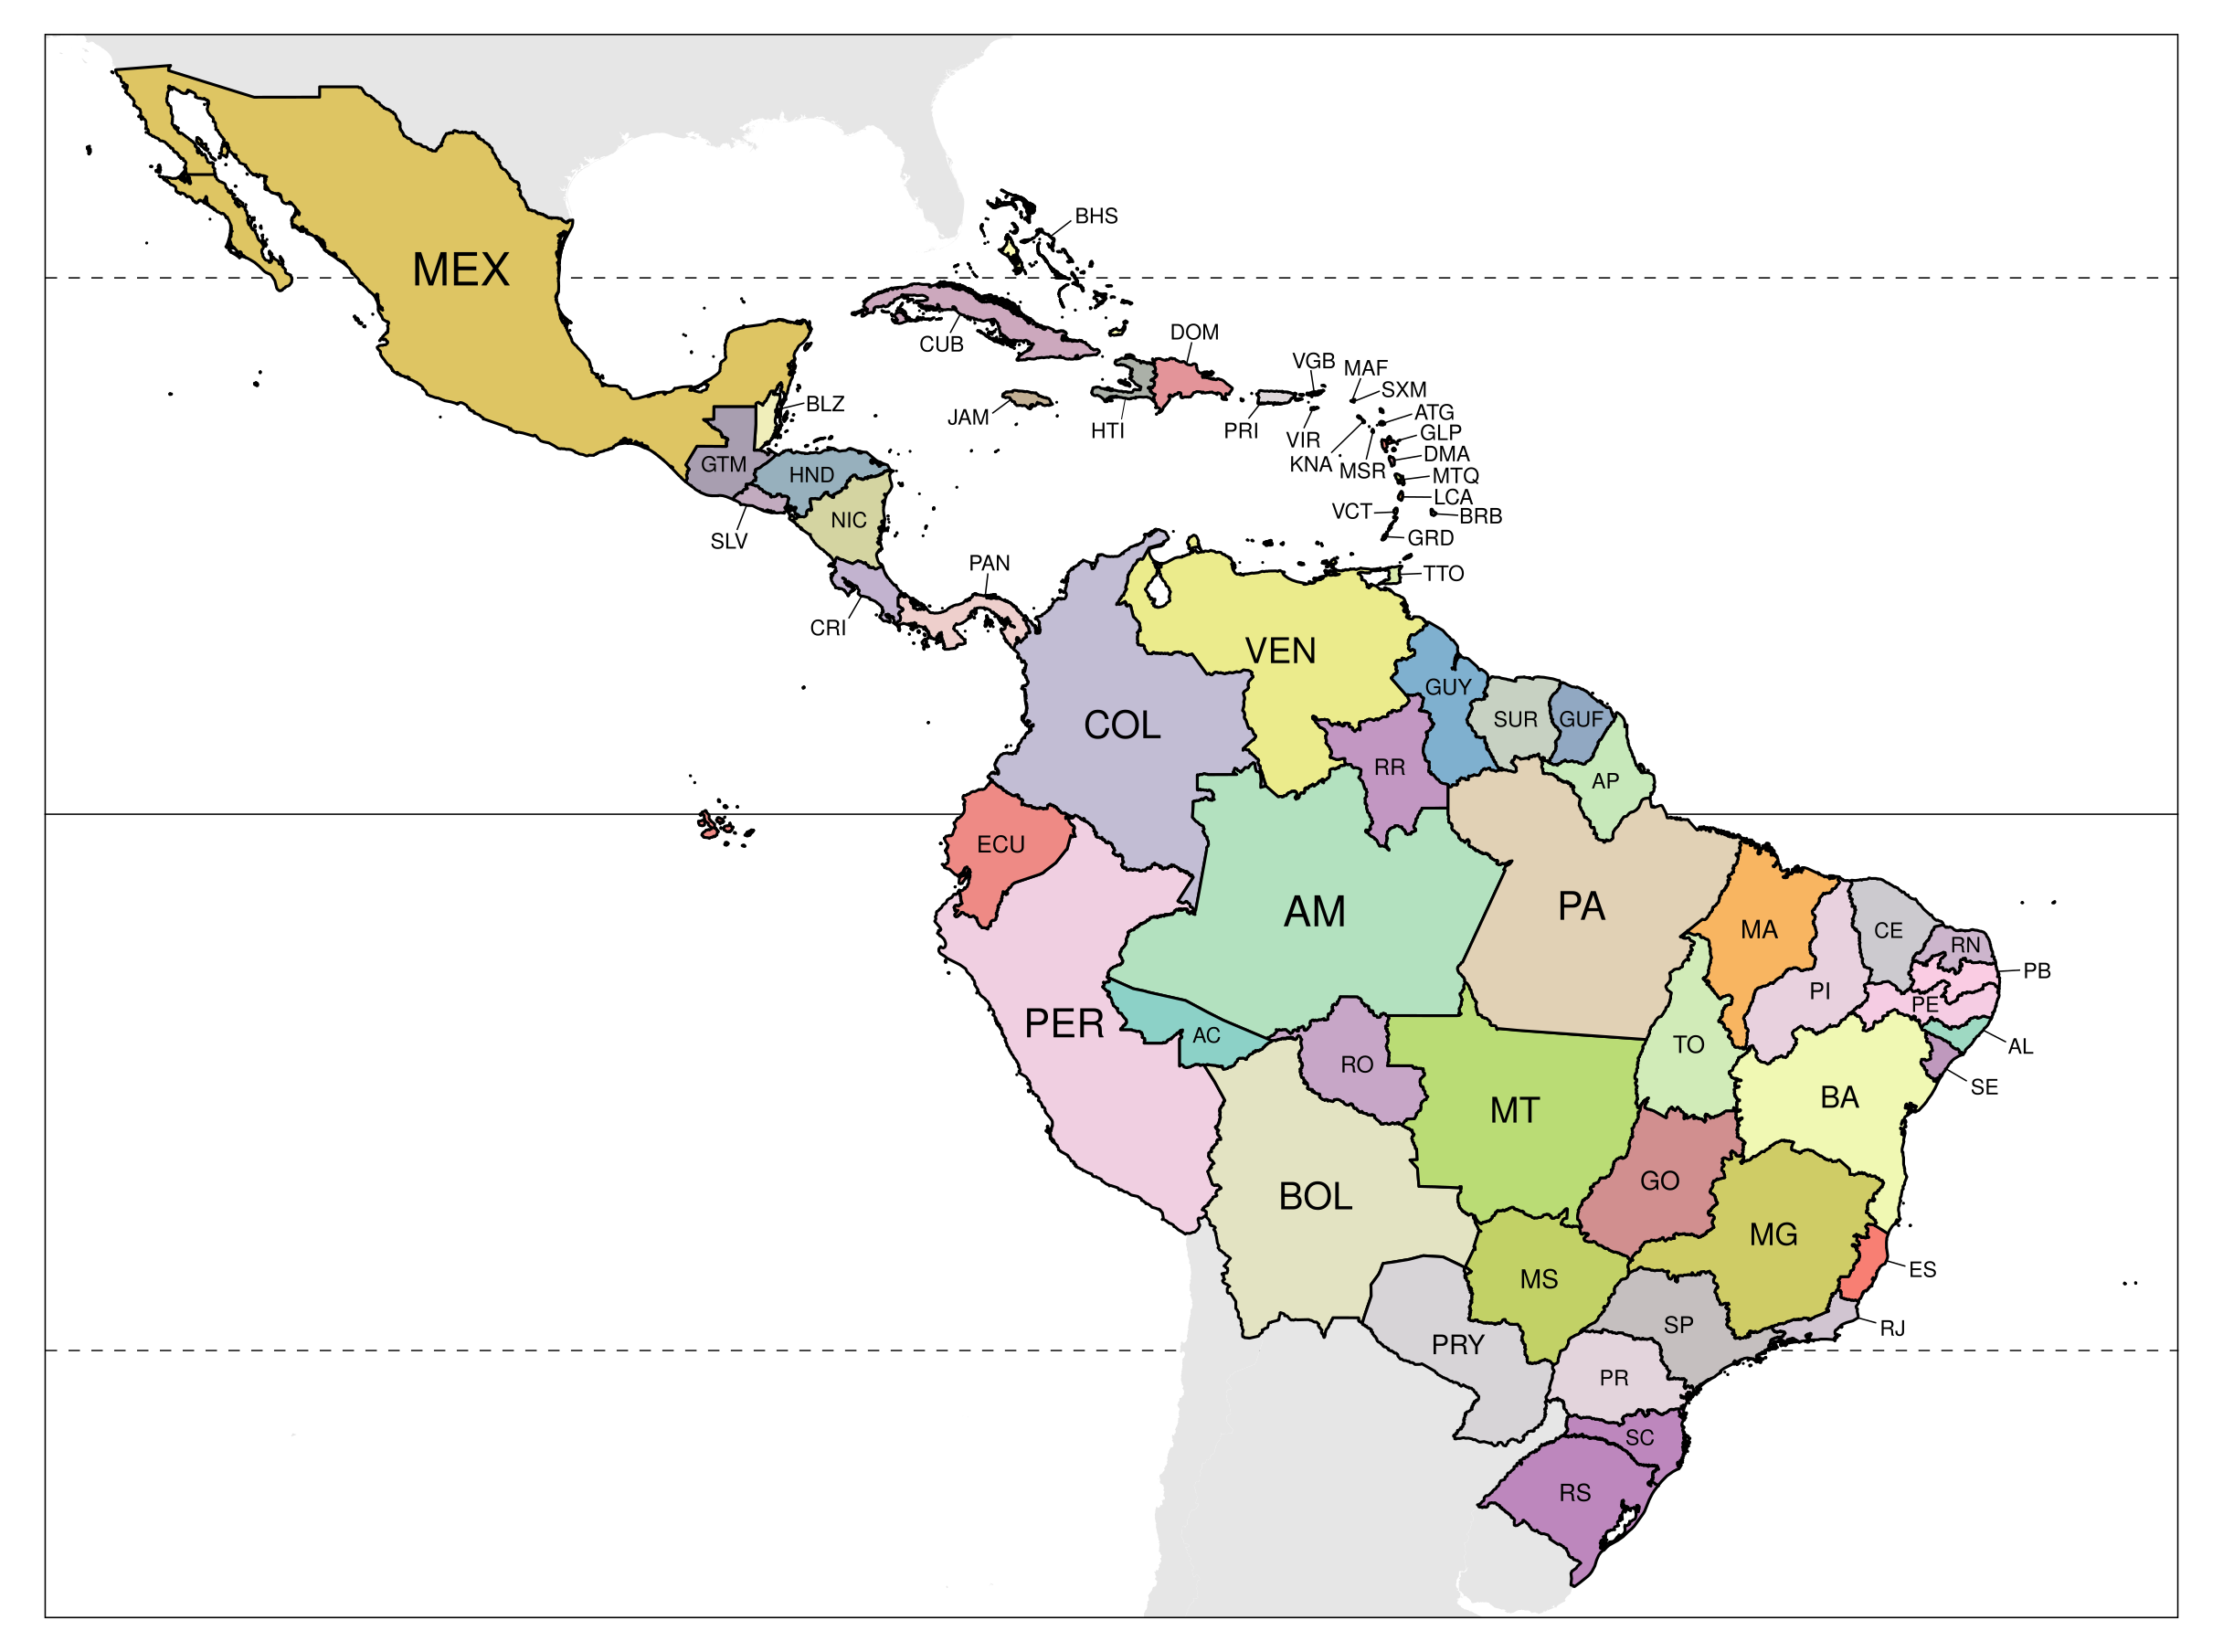
\includegraphics[width=\textwidth]{figures/study_areas_America_ink} \end{center}

\begin{center}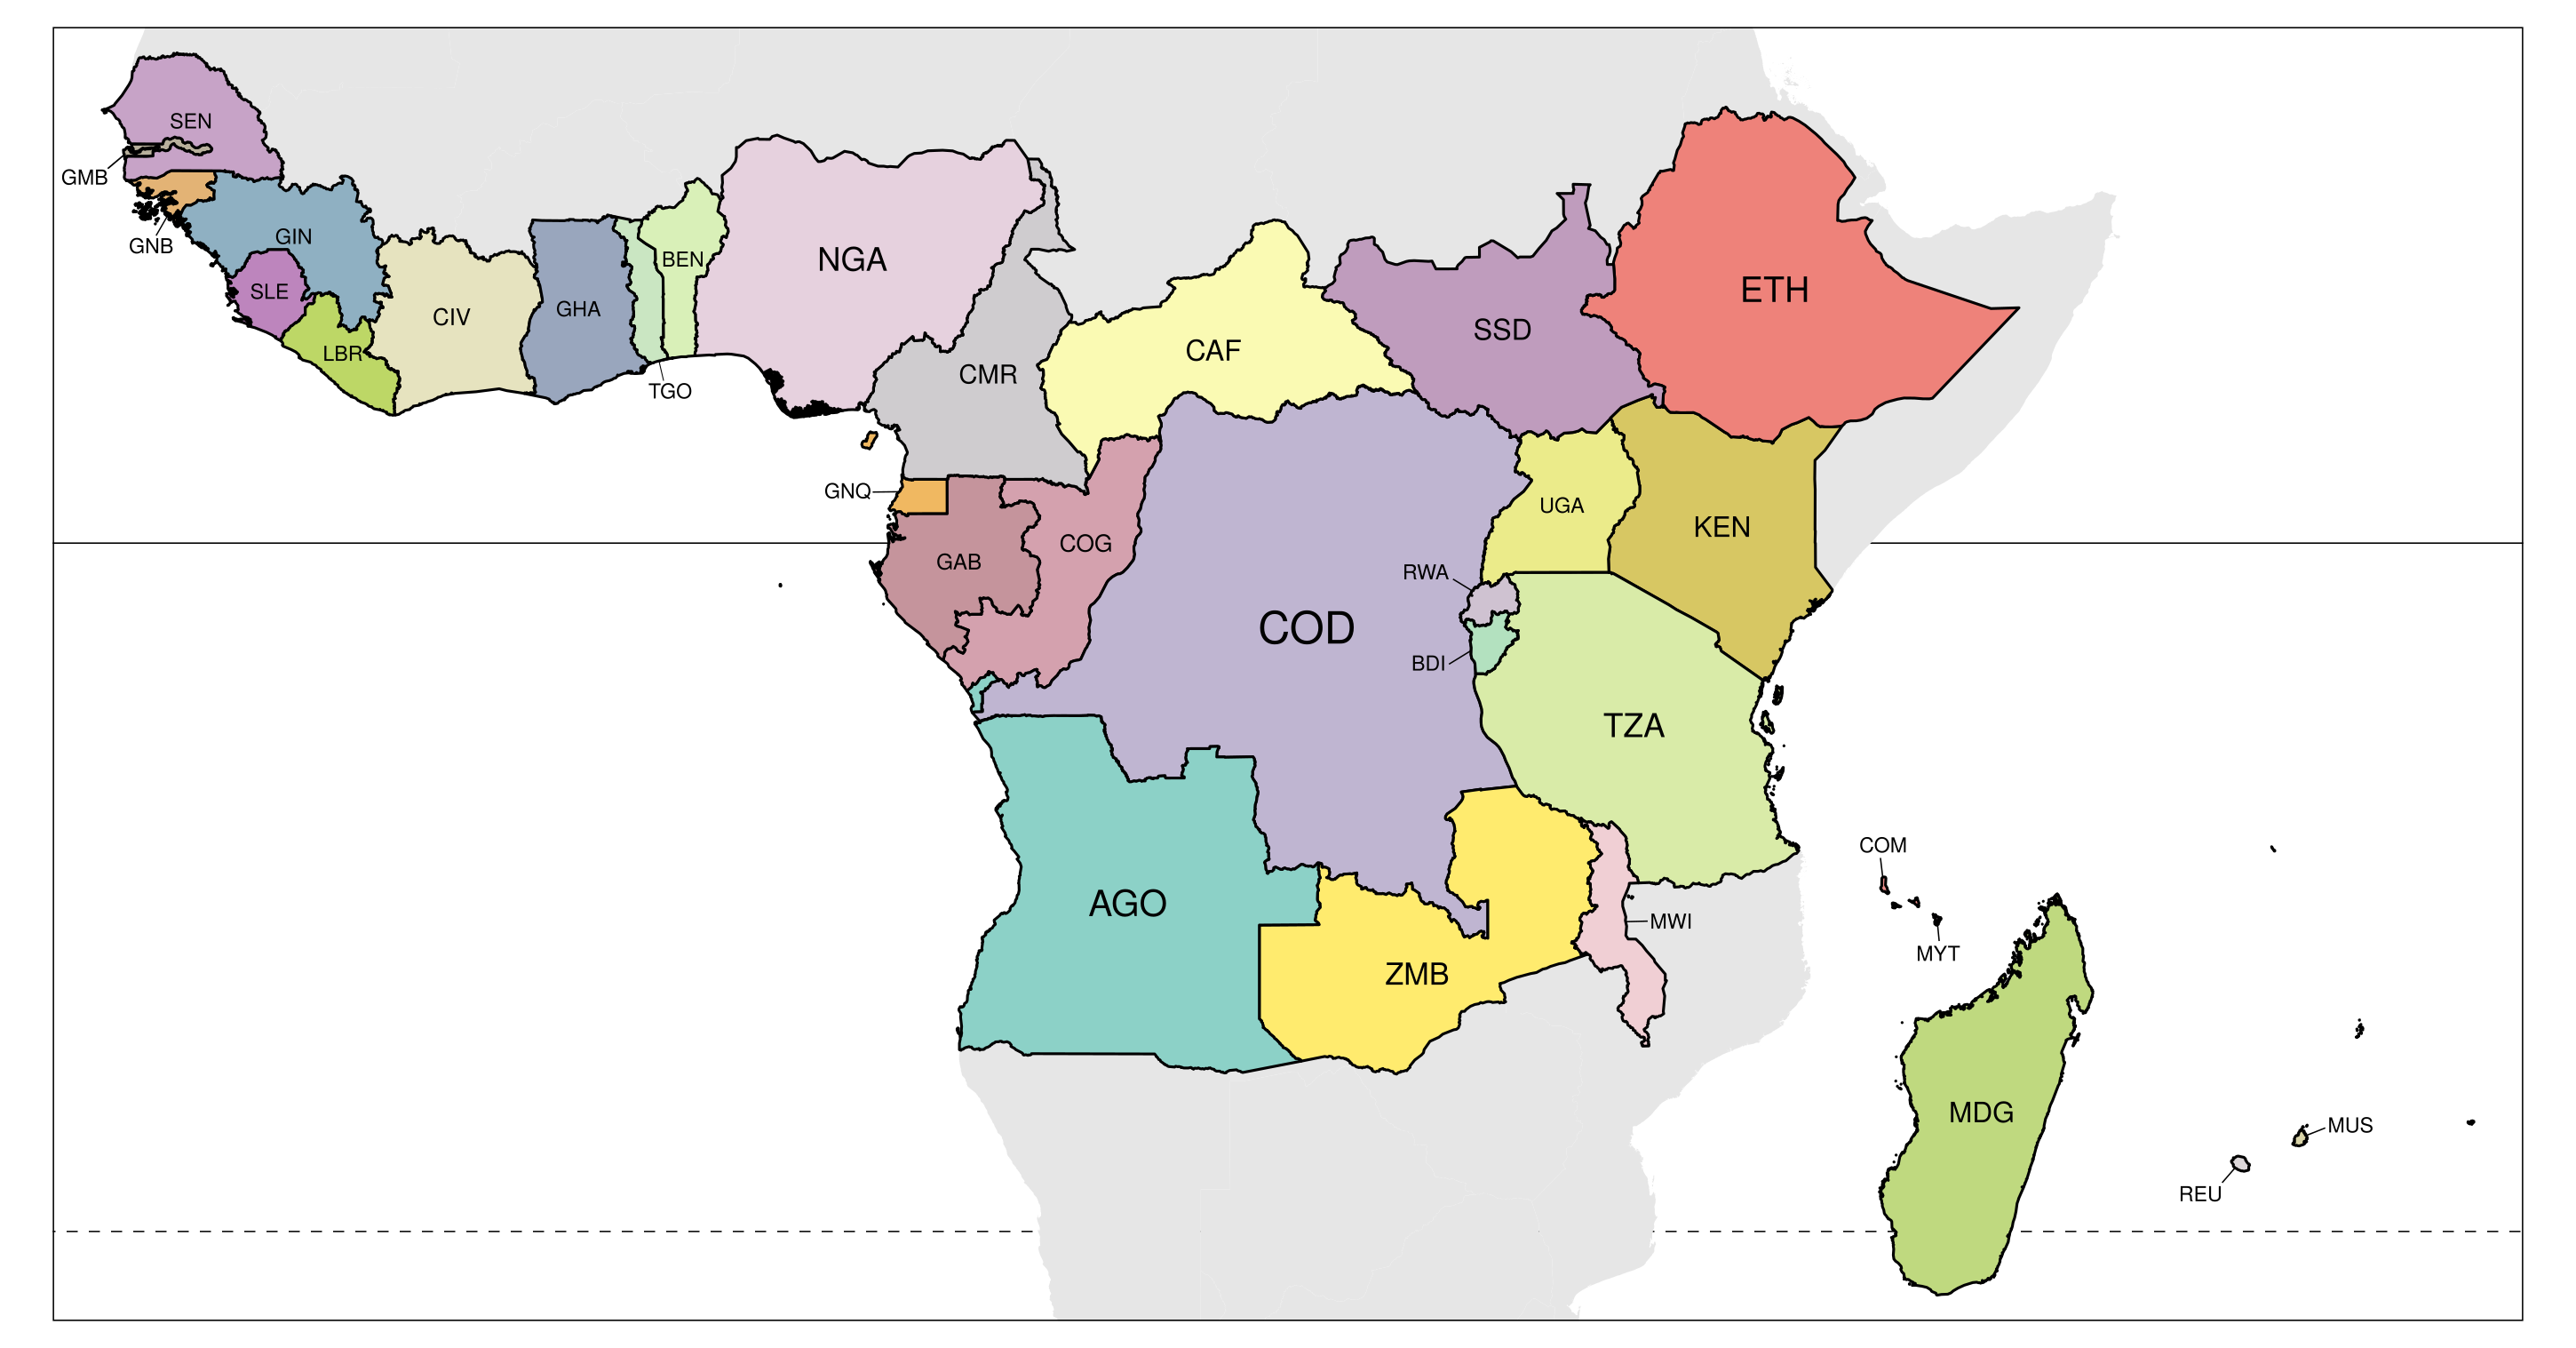
\includegraphics[width=\textwidth]{figures/study_areas_Africa_ink} \end{center}

\begin{figure}[H]

{\centering 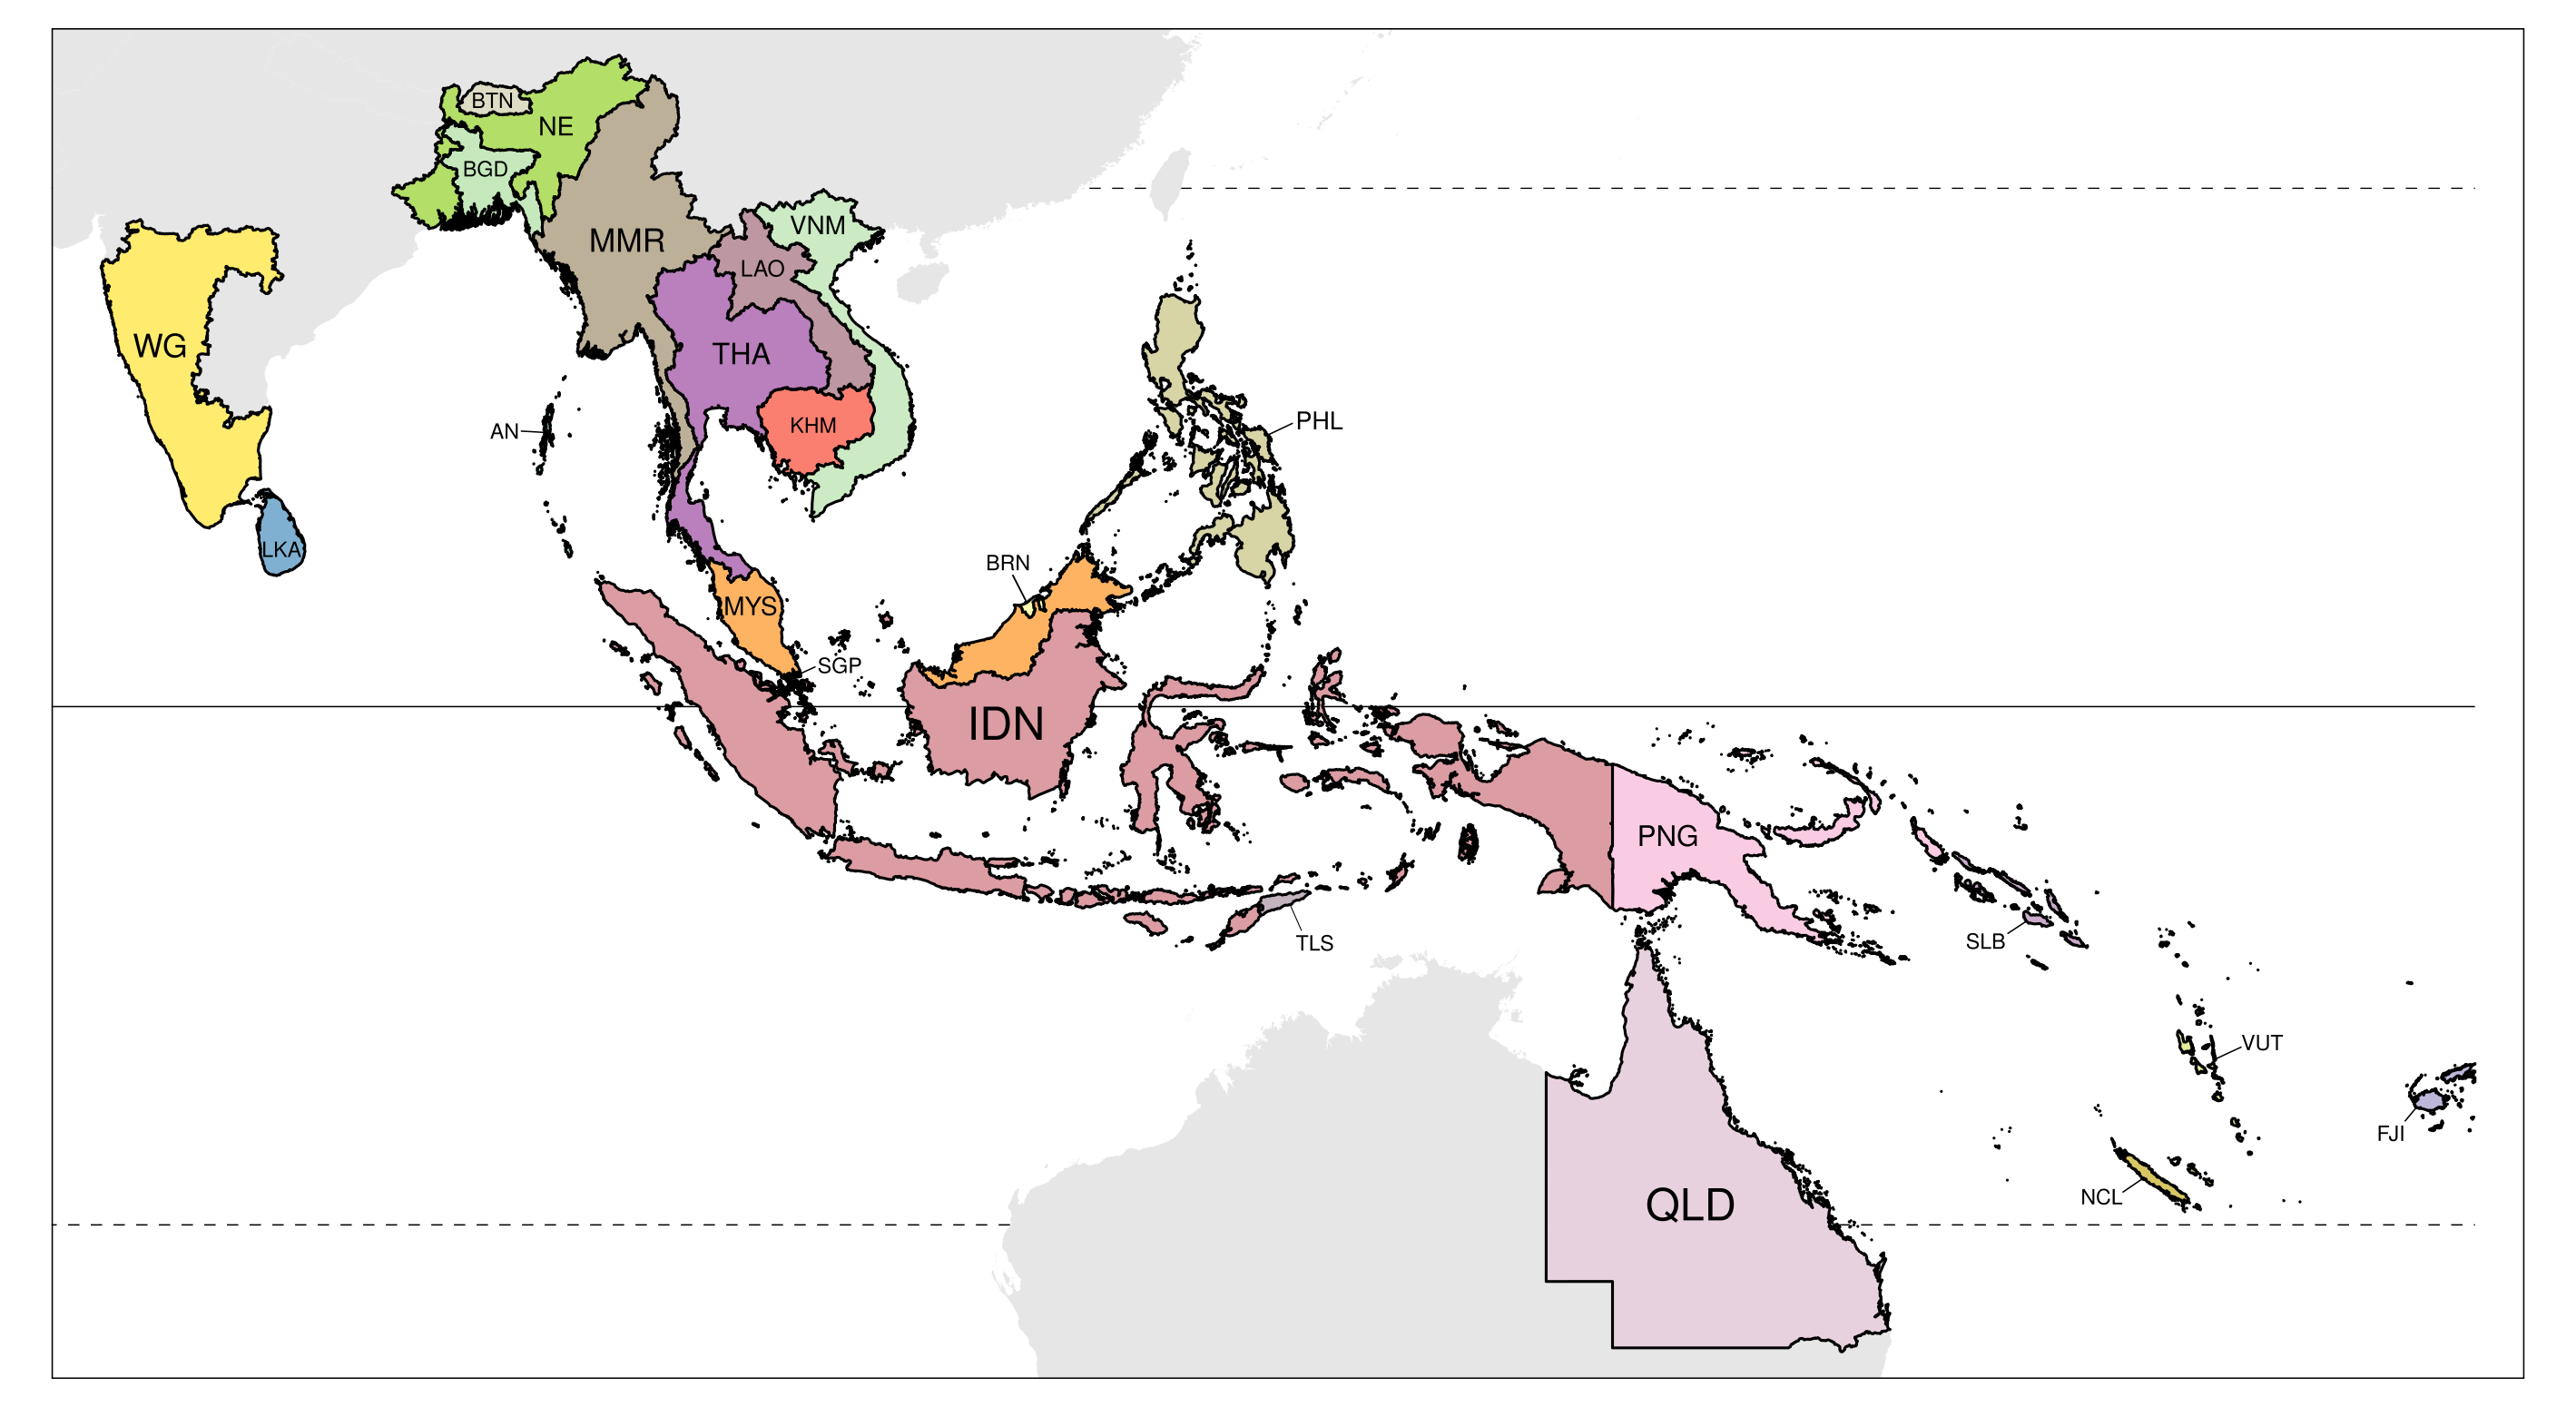
\includegraphics[width=\textwidth]{figures/study_areas_Asia_ink} 

}

\caption{\textbf{Study areas in the three continents: America, Africa, and Asia}. America included 64 study areas (39 countries), Africa included 32 study areas (32 countries), and Asia included 23 study areas (21 countries). Each country was identified by one unique three-letter code following the ISO 3166-1 standard (eg. MDG for Madagascar or GUF for French Guyana). In America, Brazil was divided in 26 study areas corresponding to the 26 Brazilian states. Each Brazilian state was defined by one unique two-letter code (eg. AM for Amazonas). For India, three study areas were considered: the Whestern Ghats (WG), the North-East India (NE), and the Andaman and Nicobar Islands (AN). For Australia, we only considered the Queensland (QLD) state as a study area. In the three figures, each study area is identified by one unique code and a set of polygons with the same color. The horizontal lines on each figure indicate the position of the Equator (plain line) and the two tropics (Cancer at the North and Capricorn at the South, dashed lines).}\label{fig:study-areas}
\end{figure}

\newpage

\hypertarget{references}{%
\section*{References}\label{references}}
\addcontentsline{toc}{section}{References}

\bibliography{/home/ghislain/Documents/Bibliography/biblio.bib}

\end{document}
